%%-*- TeX-master: t; -*-
\documentclass{article}
\usepackage{cancel,leonine,amsmath,amssymb,amsthm,graphicx, setspace}%%xy, setspace, amscd (commutative diagram)
\title{Stochastic Shape Grammars: A Comprehensible Introduction?}
\author{Eric Purdy \footnote{Department of Computer Science, University of Chicago. Email: epurdy@uchicago.edu}}


\def\ind{\mathbf{1}}

%%\doublespace

\newcommand\Inner{\mathbb{I}}
\newcommand\Outer{\mathbb{O}}
\newcommand\Full{\mathbb{F}}
% \DeclareMathOperator*\Inner{Inner}
% \DeclareMathOperator*\Outer{Outer}
% \DeclareMathOperator*\Full{Full}

\begin{document}
\maketitle

\section{Stochastic Shape Grammars}

We will represent a placed symbol $X_{p,q}$ as a labeled line segment:
\mar{labeled line segment}

We will represent a placed terminal symbol $\ell_{p,q}$ as a labeled
line segment whose line is darker.
\mar{labeled line segment}

We will represent a placed curvilinear form by chaining together
labeled line segments. Note that a curvilinear form can consist of a
mixture of placed nonterminal symbols (light lines) and placed
terminal symbols (dark lines).
\mar{labeled curvlinear form}

\mar{Describe depicted grammar}

\begin{figure}
\includegraphics[width=4.0in]{images/grammar-state.eps}
\end{figure}

\begin{figure}
\includegraphics[width=4.0in]{images/grammar-rules.eps}
\end{figure}

\section{Parse trees and Inference}

Given a placed symbol $X_{p,q}$, the PCFSG defines a distribution over
concrete substitution rules that can be applied:
\begin{align*}
  P_{sub}( \langle X_{p,q} \to Y_{p,m} Z_{m,q}\rangle ; X_{p,q})
  &= \rho_X([X\to YZ]) \cdot \mu_{X\to YZ}(m; p,q)\\
  P_{sub}( \langle X_{p,q} \to \ell_{p,q} \rangle ; X_{p,q}) 
  &= \rho_X([X\to \ell]).
\end{align*}

We can then define $P(C; \GGG, p,q)$ to be the probability that we
arrive at $C$ by starting with $S_{p,q}$ and repeatedly applying a
random concrete substitution rule according to $P_{sub}$. For a fixed
grammar $\GGG$ and a given curve $C$ with points $C[0], \dots, C[n]$,
there are potentially many ways for this sampling process to produce
$C$. In this section, we formalize this by defining parse trees.

\subsection{Preliminaries}

\begin{defn}
We define the set $\FFF_\GGG$ to be the set of all strings of placed
symbols $X^{(1)}_{p_0,p_1} X^{(2)}_{p_1,p_2} \dots X^{(k)}_{p_{k-1},
  p_k}$ with $X^{(i)} \in \NNN$, where neighboring placed symbols
$X^{(i)}_{p_{i-1},p_i} X^{(i+1)}_{p_i,p_{i+1}}$ are constrained to
share the point $p_i$.
\end{defn}

Let $C$ be a curve of length $n$, with points $C[0]$ through
$C[n]$. Since $C$ is fixed, we will abuse notation throughout this
section by writing placed symbols $X_{C[i],C[j]}$ as $X_{ij}$.

We will write a binary tree with root node $v$, left subtree $T_1$,
and right subtree $T_2$ as $\frac{v}{T_1\qquad \mid \qquad T_2}.$

\begin{defn}
  Let $T_1, T_2$ be labeled binary trees, where $u$ is a leaf node of
  $T_1$ and $v$ is the root node of $T_2$. We define a new tree $T_1
  \triangle^{\cancel{u}}_v T_2$ to be the tree resulting from deleting
  $u$ and attaching $T_2$ in its place.
\end{defn}

We differentiate between \emph{abstract substitutions}, which we will write
as $[X\to YZ]$ or $[X\to \ell]$ and \emph{concrete substitutions},
which we will write as $\langle X_{ik} \to Y_{ij} Z_{jk} \rangle$ or
$\langle X_{i i+1} \to \ell_{i i+1} \rangle$.

\subsection{Parse Trees}

\begin{defn}
  A $\GGG$-parse tree is a binary tree $T$ that specifies a sequence
  of concrete substitution rules that take some placed symbol $X_{ij}$
  to some placed curvilinear form $\lambda$.

  $T$ has three kinds of nodes:
  \begin{itemize}
  \item Unexpanded nodes, which are labeled with a placed symbol
    $X_{ij}$, where $0\le i < j \le n$ and $X\in \NNN$. Unexpanded
    nodes are always leaves.
  \item Lexical nodes, which are labeled with a concrete substitution
    rule $$\langle X_{i i+1} \to \ell_{i i+1}\rangle,$$ where $[X\to \ell]\in
    \RRR(X)$. Lexical nodes are always leaves.
  \item Binary nodes, which are labeled with a concrete substitution
    rule $$\langle X_{ik}\to Y_{ij} Z_{jk}\rangle,$$ where $X,Y,Z\in
    \NNN, [X\to YZ]\in \RRR(X)$, and $0 \le i < j < k \le n$. Binary
    nodes always have two children. The first must be either of the
    form $\langle Y_{ij} \to \lambda \rangle$ or of the form $Y_{ij}$.
    The second must be either of the form $\langle Z_{jk} \to \lambda
    \rangle$ or of the form $Z_{jk}$.
  \end{itemize}
\end{defn}
\mar{put picture of parse tree here}

To simplify notation, we will define $sym(v)$ as:
\begin{itemize}
\item $sym(X_{ij}) = X_{ij}$
\item $sym(\langle X_{i i+1} \to \ell_{i i+1}\rangle) = X_{i i+1}$
\item $sym(\langle X_{ik} \to Y_{ij} Z_{jk}\rangle) = X_{i k}$
\end{itemize}

\begin{prop}
  For $X\in \NNN, p,q\in \RR^2$, the set of all $\GGG$-parse trees $T$
  such that $sym(root(T)) = X_{p,q}$ is in one-to-one correspondence
  with the set of all derivations of placed curvilinear forms from the
  placed symbol $X_{p,q}$ according to the substitution rules of
  $\GGG$.
\end{prop}
\begin{proof}
\mar{give proof}
\end{proof}

\begin{defn}
The \emph{weight} of a parse tree $T$ is defined to be
$$ W_\GGG(T) = \prod_{\langle X_{ij} \to \lambda \rangle\in T} P_{sub}(
\langle X_{ij} \to \lambda \rangle).$$ Note that this product omits
the unexpanded nodes of $T$.
\end{defn}

We do not call this a probability because two different parse trees
are not always mutually exclusive events (in particular, if one is a
subset of the other), and thus the sum of $W_\GGG(T)$ can be greater
than one.

\begin{obs}
Let $T_1$ be a parse tree with an unexpanded leaf node $X_{ij}$, and let
$T_2$ be a parse tree with root node of the form $\langle X_{ij} \to
\lambda \rangle$. If we define
$$T = T_1 \triangle^{\cancel{X_{ij}}}_{\langle X_{ij} \to \lambda
  \rangle} T_2,$$
then
\begin{enumerate}
\item $T$ is a valid parse tree.
\item $$W_\GGG(T) = W_\GGG(T_1) W_\GGG(T_2).$$
\end{enumerate}
\end{obs}

\subsection{Inner Parse Trees}

\mar{calling it a parse tree ``of $C$'' may mislead?}
\begin{defn}
  An \emph{inner parse tree} of $C$ is a parse tree $T$ in which every
  leaf node is a lexical node. Let $\Inner_\GGG^C(X_{ij}, \lambda)$ be
  the set of all inner parse trees of $C$ with root node of the form
  $\langle X_{ij} \to \lambda \rangle$. Let $\Inner_\GGG^C(X_{ij})$ be
  the set of all inner parse trees of $C$ with root node of the form
  $\langle X_{ij} \to \lambda \rangle$ for any $\lambda \in \FFF_\GGG$.
\end{defn}

\begin{prop}
\label{prop-induct-inside}
We can construct the set $\Inner_\GGG^C(X_{ij}, \lambda)$ recursively
as follows:
\begin{itemize}
\item $\Inner_\GGG^C(X_{i i+1}, \ell_{i i+1}) = \left\{ \frac{ \langle
      X_{i i+1} \to \ell_{i i+1} \rangle}{ \emptyset \qquad \mid
      \qquad \emptyset } \right\}$
if $[X\to \ell] \in \RRR(X)$, and empty otherwise.
\item 
$    \Inner_\GGG^C(X_{ij}, Y_{ik} Z_{kj}) = \Bigg\{ \frac{\langle
  X_{ij} \to Y_{ik}Z_{kj} \rangle}{ T_Y \qquad \mid \qquad T_Z} : 
 T_Y\in
      \Inner_\GGG^C(Y_{ik}), T_Z \in \Inner_\GGG^C(Z_{kj}) \Bigg\}.
$
\end{itemize}
\end{prop}
\begin{proof}
  Let $T\in \Inner_\GGG^C(X_{ij})$. The root node is either of the
  form $\langle X_{i i+1} \to \ell_{i i+1}\rangle$ or $\langle X_{i
    j}\to Y_{i k} Z_{k j}\rangle$. In the former case, the root is a lexical
  node, and cannot have any children.

  In the latter case, since $T$ is an inner parse tree, the root node
  cannot be a leaf node, and it is constrained to have exactly two
  children, which must be of the form $\langle Y_{ik}\to
  \lambda_Y\rangle$ and $\langle Z_{kj} \to \lambda_Z \rangle$, since
  $T$ has no unexpanded nodes. Every leaf node of either subtree is
  also a leaf node of $T$, and thus lexical. Therefore the subtrees
  headed by these nodes are also inner parse trees, and reside in the
  specified sets.
\end{proof}

\begin{prop}
\label{prop-inside-corr}
  The set $\Inner_\GGG^C(X_{ij})$ is in one-to-one correspondence with
  the set of derivations of $C[i:j]$ from the placed symbol $X_{ij}$
  according to the substitution rules of $\GGG$. Moreover, $W_\GGG(T)$
  gives the probability of the derivation.
\end{prop}
\begin{proof}
\mar{give proof}
\end{proof}

The probability that we derive a curve $C[i:j]$ from a placed symbol
$X_{ij}$ is just the sum of the probabilities of any particular
derivation, taken over all possible derivations. This probability is
called the \emph{inside probability}:
$$Inside_\GGG^C(X_{i j}) =  \sum_{T\in \Inner_\GGG^C(X_{ij})}W_\GGG(T).$$
Since $P(C\mid \GGG)$ is just the total probability of deriving $C$
from $\GGG$, it is clear by Proposition \ref{prop-inside-corr} that 
$$P(C\mid \GGG) = Inside_\GGG^C(S_{0 n}).$$

We can compute the inside probability efficiently:

\begin{obs}
We can compute all inside probabilities in time $O(|\RRR|n^3)$ by using the
following relations:
  \begin{align*}
Inside_\GGG^C(X_{i i+1}) &= \sum_{T\in \Inner_\GGG^C(X_{i i+1})}
W_\GGG(T)\\
 &= P_{sub}(\langle X_{i i+1} \to \ell_{i i+1} \rangle) \\
\intertext{by the first case of Propostion \ref{prop-induct-inside}.}
Inside_\GGG^C(X_{ij}) &= \sum_{T\in \Inner_\GGG^C(X_{ij})} W_\GGG(T)\\
&= \sum_{\substack{[X\to YZ] \in \RRR(X)\\ i < k < j}} \sum_{T\in
  \Inner_\GGG^C(X_{ij}, Y_{ik}Z_{kj})} W_\GGG(T)\\
\intertext{by the definition of $\Inner_\GGG^C(X_{ij})$}
&= \sum_{\substack{[X\to YZ] \in \RRR(X)\\ i < k < j}} 
P_{sub}(\langle X_{ij} \to Y_{ik} Z_{kj} \rangle)
\sum_{T_Y\in \Inner_\GGG^C(Y_{ik})}
\sum_{T_Z\in \Inner_\GGG^C(Z_{kj})}
 W_\GGG(T_Y) W_\GGG(T_Z)\\
\intertext{by the second case of Propostion \ref{prop-induct-inside}}
&= \sum_{\substack{[X\to YZ] \in \RRR(X)\\ i < k < j}} 
P_{sub}(\langle  X_{ij} \to Y_{ik} Z_{kj} \rangle)
Inside_\GGG^C(Y_{ik})
Inside_\GGG^C(Z_{kj})
  \end{align*}
\end{obs}

\subsection{Outer Parse Trees}

\begin{defn}
  An \emph{outer parse tree} of $C$ is a parse tree $T$ with
  $sym(root(T)) = S_{0n}$ in which one special leaf is an unexpanded node
  $X_{ij}$, and all other leaf nodes are lexical nodes. Let
  $\Outer_\GGG^C(X_{ij})$ be the set of all outer parse trees which
  have unexpanded node $X_{ij}$.
\end{defn}

\begin{prop}
  We can construct the set $\Outer_\GGG^C(X_{ij})$ recursively as
  follows:
\begin{itemize}
\item $\Outer_\GGG^C(X_{0n}) = \left\{ \frac{S_{0n}}{\emptyset \qquad
      \mid \qquad \emptyset} \right\}$, if $X=S$, and is empty otherwise.
\item 
\begin{align*}
&\Outer_\GGG^C(X_{ij}) = \\
&\bigcup_{\substack{h < i \\ [Z \to YX]\in \RRR}}
\Bigg\{
T_{out} \triangle^{\cancel{Z_{hj}}}_{\langle Z_{hj} \to Y_{hi}
  X_{ij})\rangle} \frac{ \langle Z_{hj} \to Y_{hi}
  X_{ij} \rangle}{ T_Y \qquad \mid \qquad X_{ij}} : \\
&\qquad\qquad\qquad T_{out} \in \Outer_\GGG^C(Z_{hj}), T_Y \in \Inner_\GGG^C(Y_{hi}) 
\Bigg\} \bigcup\\
&\bigcup_{\substack{i < k \\ [Z \to
    XY]\in \RRR}}
\Bigg\{
T_{out} \triangle^{\cancel{Z_{ik}}}_{\langle Z_{ik} \to X_{ij} Y_{jk}
  \rangle} \frac{ \langle Z_{ik} \to X_{ij}
  Y_{jk} \rangle}{ X_{ij} \qquad \mid \qquad  T_Y } :\\
&\qquad\qquad\qquad T_{out} \in \Outer_\GGG^C(Z_{ik}),
 T_Y \in \Inner_\GGG^C(Y_{jk}) \Bigg\}\\
\end{align*}
(For notational simplicity above, we are writing $X_{ij}$ in
place of $\frac{X_{ij}}{\emptyset \qquad \mid \qquad
  \emptyset}$.)
\end{itemize}
\end{prop}
\begin{proof}
  Let $T\in \Outer_\GGG^C(X_{ij})$. The unexpanded
  node $X_{ij}$ may be the root of $T$, in which case $X_{ij}$ must be
  $S_{0n}$, and we are in the first case.

  Otherwise, $X_{ij}$ is not the root of $T$, and has a parent which
  is either $\langle Z_{hj} \to Y_{hi} X_{ij} \rangle$, or $\langle
  Z_{ik} \to X_{ij} Y_{jk} \rangle$. Let us restrict to the second
  case; the first case is strictly analogous. 
  
  If we remove the subtree rooted at $Y_{jk}$ and replace $\langle
  Z_{ik} \to X_{ij} Y_{jk} \rangle$ with an unexpanded node $Z_{ik}$, we get a
  tree $T_{out}$ which is a valid outer tree for $Z_{ik}$:
  \begin{itemize}
  \item $T_{out}$ has a single unexpanded node $Z_{ik}$
  \item $root(T_{out}) = root(T) = S_{0n}$.
  \end{itemize}
  Furthermore, the subtree $T_Y$ rooted at $Y_{jk}$ satisfies
  $sym(root(T_Y)) = Y_{jk}$, and is an inner parse tree, since all
  remaining leaf nodes are lexical nodes. This completes the proof.
  
\end{proof}

We define the \emph{outside weight} as:
$$Outside_\GGG^C(X_{ij}) = \sum_{T\in \Outer_\GGG^C(X_{ij})}
W_\GGG(T).$$ This gives the total weight of parse trees corresponding
to derivations of the curvilinear form $\ell_{C[0], C[1]}\dots
\ell_{C[i-1],C[i]} X_{ij} \ell_{C[j], C[j+1]} \dots \ell_{C[n-1],
  C[n]}$ from $S_{0n}$.

\begin{obs}
  Given the inside probabilities, we can compute the outside weights
  in time $O(|\RRR| n^3)$ by using the following relations:
  \begin{align*}
    Outside_\GGG^C(S_{0n}) &= \sum_{T\in \Outer_\GGG^C(S_{0n})}
    W_\GGG(T) \\
&= W_\GGG\left(\frac{S_{0n}}{\emptyset \qquad \mid \qquad
    \emptyset}\right) = 1\\
\intertext{by the first case of Proposition \ref{2.12}.}
Outside_\GGG^C(X_{ij}) 
&= \sum_{T\in \Outer_\GGG^C(X_{ij})}
    W_\GGG(T) \\
&=
 \sum_{\substack{h < i \\ [Z\to YX] \in
    \RRR}} P_{sub}(\langle Z_{hi} \to Y_{hi}X_{ij} \rangle)
\sum_{T_{out}\in \Outer_\GGG^C(Z_{hj})}
\sum_{T_{Y}\in \Inner_\GGG^C(Y_{hi})}
W_\GGG(T_{out}) W_\GGG(T_Y)\\
&+
 \sum_{\substack{j<k \\ [Z\to XY] \in
    \RRR}} P_{sub}(\langle Z_{ik} \to X_{ij}Y_{jk} \rangle)
\sum_{T_{out}\in \Outer_\GGG^C(Z_{ik})}
\sum_{T_{Y}\in \Inner_\GGG^C(Y_{jk})}
W_\GGG(T_{out}) W_\GGG(T_Y)
\intertext{by the second case of Proposition \ref{2.12}.}
&= 
 \sum_{\substack{h < i \\ [Z\to YX] \in
    \RRR}} P_{sub}(\langle Z_{hi} \to Y_{hi}X_{ij} \rangle)
Outside_\GGG^C(Z_{hj}) Inside_\GGG^C(Y_{hi})\\
&+
 \sum_{\substack{j<k \\ [Z\to XY] \in
    \RRR}} P_{sub}(\langle Z_{ik} \to X_{ij}Y_{jk} \rangle)
Outside_\GGG^C(Z_{ik}) Inside_\GGG^C(Y_{jk})
  \end{align*}
\end{obs}

\subsection{Dealing with Closed Curves}

When we are dealing with a closed curve $C$, the machinery of the
preceding sections does not work as is. For example, there is no
reason why parse trees should necessarily be rooted at $S_{0n}$, since
we can split the curve at an index other than $0$. 

In order to allow a curve to be split in other ways, we define a
rotation operation:
$$C^{\leftarrow k}[i] = C[(i-k) \mod n].$$
We think of $C$ as being a random rotation of some other closed
curve $D$, and set $P(C = D^{\leftarrow k}) = \frac{1}{n}$.

We can then treat the closed curve $D[0], \dots, D[n-1]$ as an open
curve $D[0], \dots, D[n-1], D[n]=D[0]$ whose endpoints happen to be
the same.

\begin{rmk}
  For closed curve grammars, the top-level midpoint distributions
  $\mu_{S\to XY}$ cannot be proper distributions if our grammar is
  going to be invariant under similarity transformations (translation,
  scaling, and rotation). This is because any choice of midpoint is
  equally good, since we can map any pair $(p,q)$ to any other pair
  $(p',q')$ via a similarity transformation. This is a problem
  because we cannot define a uniform distribution on all of $\RR^2$!

  We handle this by setting $\mu_{S\to XY}(\cdot) = 1$ in our
  formulas. We justify this by thinking of each curve as being a
  representative of its equivalence class under similarity
  transformations.  
\end{rmk}


The probability that we see a parse tree is therefore $P(C,T\mid \GGG)
= \frac{1}{n} W_\GGG(T).$ The inside weights are unaffected by this
change - once we specify the root node $X_{ij}$, it is irrelevant
which shift of $C$ is being examined. (Although some shifts will not
allow $X_{ij}$, since $C[j]$ will be to the left of $C[i]$.)

The outside weights are affected by the change. For each $k$ such that
$0\le k < n$, we have a distinct $Outside_\GGG^{C^{\leftarrow
    k}}(X_{ij})$.
We can simplify matters by defining 
$$COutside_\GGG^C(X_{ij}) = \frac{1}{n} \sum_k
Outside_\GGG^{C^{\leftarrow k}}(X_{(i + k \mod n) (j + k \mod n)}).$$

\begin{prop}
We can compute $COutside_\GGG^C(X_{ij})$ recursively as follows:
$$COutside_\GGG^C(S_{ii}) = \frac{1}{n}.$$

\begin{align*}
COutside_\GGG^C(X_{ij}) &=
   \sum_{\substack{h < i \\ [Z\to YX] \in
    \RRR}} P_{sub}(\langle Z_{hi} \to Y_{hi}X_{ij} \rangle)
COutside_\GGG^C(Z_{hj}) Inside_\GGG^C(Y_{hi})\\
&+
 \sum_{\substack{j<k \\ [Z\to XY] \in
    \RRR}} P_{sub}(\langle Z_{ik} \to X_{ij}Y_{jk} \rangle)
COutside_\GGG^C(Z_{ik}) Inside_\GGG^C(Y_{jk})
\end{align*}
\end{prop}
\begin{proof}
\mar{finish and prove by induction.}
We proceed by downwards induction on the length of $X_{ij}$. The value
for $COutside_\GGG(S_{ii})$ is straight from the definition.

\end{proof}

\section{EM}

Let $C_1,\dots, C_n$ be independent samples from a grammar $\GGG$, for
which we know the structure, but not the parameters. We would like to
set the parameters of $\GGG$ such that the posterior $P(\GGG\mid
C_1,\dots,C_n)$ is maximized. We can write the posterior as
\begin{align*}
  P(\GGG\mid C_1,\dots, C_n) &= P(\GGG) \cdot \prod_i P(C_i\mid \GGG)\\
  &= P(\GGG) \cdot \prod_i \sum_{T\in Parse_\GGG(C_i)}P(C_i, T \mid \GGG)\\
  &= P(\GGG) \cdot \sum_{\{T_i\}}\prod_i P(C_i, T_i \mid \GGG)\\
\end{align*}
Unfortunately, it is not known how to maximize this posterior, or even
the likelihood. The likelihood is known to have many local maxima in
the case of context-free grammars for natural languages
\cite{charniak}. Therefore, we are forced to use approximation
techniques. We use the Expectation-Maximization algorithm \cite{em},
which is a standard approach to finding maximum likelihood or maximum
a posteriori estimates in the case where important variables are
unobserved. In our case, the unobserved variables are the parse trees
$\{T_i\}$.

Let $\mathbf{C} = (C_1,\dots,C_n)$, and let $\mathbf{T}$ be the latent
variable $(T_1,\dots,T_n)$. We then iteratively find better and better
grammars $\GGG^{(t)}$:
\begin{enumerate}
\item \textbf{E step:} Let 
  \begin{align*}
Q^{(t)}(\GGG) &= \sum_{\mathbf{T}} \big[P(\mathbf{T}\mid \mathbf{C},
\GGG^{(t)}) \log P(\mathbf{C},\mathbf{T}\mid \GGG) \big] + \log
P(\GGG)\\
&= E_{\mathbf{T} \sim \mathbf{T} | \mathbf{C}, \GGG^{(t)}}\big[\log
P(\mathbf{C},\mathbf{T}\mid \GGG) \big] + \log P(\GGG)
  \end{align*}
\item \textbf{M step:} Let
$$ \GGG^{(t+1)} = \argmax_{\GGG} Q^{(t)}(\GGG)$$
\end{enumerate}

\subsection{The E Step}

$$Q^{(t)}(\GGG) = E_{\mathbf{T}\sim \mathbf{T}, \GGG^{(t)}} [\log
P(C,T\mid \GGG)] + \log P(\GGG)$$
Since $P(\mathbf{C},\mathbf{T}\mid \GGG) = \prod_a P(C_a, T_a\mid \GGG),$
and by linearity of expectation:
$$Q^{(t)}(\GGG) = \sum_a E_{T_a\sim \Delta^{(t)}_a} [\log
P(C_a,T_a \mid \GGG)] + \log P(\GGG),$$
where $\Delta^{(t)}_a(T_a)$ is the distribution $P(T_a\mid C_a,
\GGG^{(t)})$.

Let $Q_a^{(t)}(\GGG) =E_{T_a \sim \Delta_a^{(t)}}[\log P(C_a,T_a\mid
\GGG)].$ We can decompose $P(C_a, T_a\mid \GGG)$ by using Proposition
\ref{prop-foo} \footnote{If $\GGG$ is a grammar for closed curves,
  $P(C_a,T_a\mid \GGG)$ will have an extra factor of
  $\frac{1}{|C|}$. We can ignore this because the logarithm turns it
  into an additive constant, which is irrelevant in the M step.}:

\begin{align*}
  Q_a^{(t)}(\GGG) &=
E_{T_a \sim \Delta_a^{(t)}}\left[\log
    \prod_{\langle X_{ij} \to \lambda\rangle \in T_a} P_{sub}(\langle
    X_{ij} \to \lambda\rangle)\right]\\
&=
E_{T_a \sim \Delta_a^{(t)}}\left[
    \sum_{\langle X_{ij} \to \lambda\rangle \in T_a} \log P_{sub}(\langle
    X_{ij} \to \lambda\rangle)\right]\\
\intertext{We can rewrite this as a sum over all possible concrete
  substitution rules, using indicator variables to eliminate absent terms:}
&=
E_{T_a \sim \Delta_a^{(t)}}\Bigg[
\sum_{i < j < k} \sum_{[X\to YZ]\in \RRR}\ind [ 
\langle X_{ik}
\to Y_{ij} Z_{jk} \rangle] \quad \log P_{sub}(\langle X_{ik} \to Y_{ij}
Z_{jk}\rangle )\\
&\qquad+\qquad \sum_{i} \sum_{[X\to \ell]\in \RRR}\ind [ \langle X_{i i+1}
\to \ell_{i i+1} \rangle] \quad \log P_{sub}(\langle X_{i i+1} \to \ell_{i i+1}\rangle)
\Bigg]\\
&=
\sum_{i < j < k} \sum_{[X\to YZ]\in \RRR} \log P_{sub}(\langle X_{ik} \to Y_{ij}
Z_{jk}\rangle ) \quad E_{T_a \sim \Delta_a^{(t)}}[\ind [ 
\langle X_{ik}
\to Y_{ij} Z_{jk} \rangle]]\\
&+ \sum_{i} \sum_{[X\to \ell]\in \RRR}
\log P_{sub}(\langle X_{i i+1} \to \ell_{i i+1}\rangle)
\quad E_{T_a \sim \Delta_a^{(t)}}[\ind [ \langle X_{i i+1}
\to \ell_{i i+1} \rangle]] 
\end{align*}
\mar{need to be more careful with indices for closed curves. basically
want clockwise}

Let 
\begin{align*}
  Count_a^{(t)}(\langle X_{ik} \to Y_{ij} Z_{jk} \rangle) &=  E_{T_a \sim \Delta_a^{(t)}}[\ind [ 
\langle X_{ik}
\to Y_{ij} Z_{jk} \rangle]]\\
&= P_{T_a \sim \Delta_a^{(t)}}( \langle X_{ik} \to Y_{ij} Z_{jk}
\rangle \in T_a)\\
Count_a^{(t)}(\langle X_{ii+1} \to \ell_{i i+1} \rangle) &=
E_{T_a \sim \Delta_a^{(t)}}[\ind [ \langle X_{i i+1}
\to \ell_{i i+1} \rangle]] \\
&= P_{T_a \sim \Delta_a^{(t)}}( \langle X_{i i+1} \to \ell_{i i+1} \rangle \in T_a)\\
\end{align*}
and let
\begin{align*}
  Q^{(t)}_{a,i,j,k,[X\to YZ]}(\GGG) &= 
\log P_{sub}(\langle X_{ik} \to Y_{ij}
Z_{jk}\rangle ) \cdot   Count_a^{(t)}(\langle X_{ik} \to Y_{ij} Z_{jk} \rangle)\\
Q^{(t)}_{a,i,[X\to \ell]}(\GGG) &=
\log P_{sub}(\langle X_{i i+1} \to \ell_{i i+1}\rangle)
\cdot Count_a^{(t)}(\langle X_{ii+1} \to \ell_{i i+1} \rangle).
\end{align*}

Since $\Delta_a^{(t)} = P(T_a \mid C_a, \GGG^{(t)})$, we can compute
it from the inside and outside weights via the following propositions:
\mar{Define $\Full$.}

\begin{prop}
Every complete $\GGG$-parse tree $T$ of $C$ containing a node
$\langle X_{ij}\to \lambda\rangle$ can be obtained as
$$T_{out} \triangle^{\cancel{X_{ij}}}_{(X_{ij},\lambda)} T_{in},$$ 
where $T_{out}\in \Outer_\GGG^C(X_{ij})$ and $T_{in} \in
\Inner_\GGG^C(X_{ij}, \lambda)$.
\end{prop}

\begin{prop}
\mar{fix this}
\begin{align*}
P(\langle X_{ij}, \lambda \rangle \in T) &=
\sum_{T \ni \langle X_{ij}, \lambda\rangle} W_\GGG(T)\\
&=
\left(\sum_{T_{out}\in \Outer_\GGG^C(X_{ij})}
  W_\GGG(T_{out}) \right)
\left(\sum_{T_{in}\in \Inner_\GGG^C(X_{ij},\lambda)} W_\GGG(T_{in})
\right)\\
&= Outside_\GGG^C(X_{ij}) Inner_\GGG^C()
\end{align*}
\end{prop}


To summarize,

\begin{centering}
\framebox{
\parbox{5in}{
\begin{align*}
  Q^{(t)}(\GGG) &= \sum_a \sum_{i,j,k} \sum_{[X\to YZ]\in \RRR}
  Q^{(t)}_{a,i,j,k,[X\to YZ]}(\GGG)\\
&+ \sum_a \sum_{i} \sum_{[X\to \ell]\in \RRR}
  Q^{(t)}_{a,i,[X\to \ell]}(\GGG)\\
&+ \log P(\GGG)
\end{align*}

\begin{align*}
  Q^{(t)}_{a,i,j,k,[X\to YZ]}(\GGG) &= 
\log P_{sub}(\langle X_{ik} \to Y_{ij}
Z_{jk}\rangle ) \cdot   Count_a^{(t)}(\langle X_{ik} \to Y_{ij} Z_{jk} \rangle)\\
Q^{(t)}_{a,i,[X\to \ell]}(\GGG) &=
\log P_{sub}(\langle X_{i i+1} \to \ell_{i i+1}\rangle)
\cdot Count_a^{(t)}(\langle X_{ii+1} \to \ell_{i i+1} \rangle) \\
\end{align*}

\begin{align*}
  Count_a^{(t)}(\langle X_{ik} \to Y_{ij} Z_{jk} \rangle) &=  E_{T_a \sim \Delta_a^{(t)}}[\ind [ 
\langle X_{ik}
\to Y_{ij} Z_{jk} \rangle]]\\
Count_a^{(t)}(\langle X_{ii+1} \to \ell_{i i+1} \rangle) &=
E_{T_a \sim \Delta_a^{(t)}}[\ind [ \langle X_{i i+1}
\to \ell_{i i+1} \rangle]] \\
\end{align*}
}
}
\end{centering}

\subsection{Potentially useful old part}
We can compute the expectation as follows: 
\begin{align*}
&=  \sum_a E_{T_a \sim T_a \mid C_a, \GGG^{(t)}}[\#\{\mbox{uses of }[X
  \to \lambda] \in T_a\}]\\
&= \sum_a \sum_{T_a \in Parse_{\GGG^{(t)}}(C_a)} P(T_a\mid C_a,
  \GGG^{(t)}) \cdot \{\mbox{uses of }[X  \to \lambda] \in T_a\}\\
&= \sum_a \sum_{T_a \in Parse_{\GGG^{(t)}}(C_a)}
\frac{P(C_a, T_a\mid \GGG^{(t)})}{P(C_a\mid \GGG^{(t)})} \cdot \{\mbox{uses of }[X
  \to \lambda] \in T_a\}
\end{align*}

\subsection{Computing Soft Counts}

We will put this in the EM section.


\subsection{The M Step}

We want to find the probabilities $p_{X,\lambda}$ for $\rho_X([X\to
\lambda])$ so that $Q^{(t)}$ is maximized.

We wish to optimize $Q^{(t)}$ with respect to the multinomial
distributions $\rho_X$ for each $X$. Let us fix $X$, and denote
$\rho_X([X\to \lambda])$ by $p_\lambda$. Then

\begin{align*}
\frac{\partial Q^{(t)}(\GGG)}{\partial p_{YZ}} &=
\sum_{a,i,j,k} \frac{\partial Q^{(t)}_{a,i,j,k,[X\to
    YZ]}(\GGG)}{\partial p_{YZ}} + \frac{\partial P(\GGG)}{\partial p_{YZ}} \\
&= 
\sum_{a,i,j,k} Count^{(t)}_a(\langle X_{ik} \to Y_{ij} Z_{jk} \rangle)
\frac{\partial \log P_{sub}(\langle X_{ik} \to
  Y_{ij}Z_{jk}\rangle)}{\partial p_{YZ}} + \frac{\partial
  P(\GGG)}{\partial p_{YZ}} \\
\intertext{Since $P_{sub}(\langle X_{ik} \to
  Y_{ij}Z_{jk}\rangle) = \rho_X([X\to YZ]) \cdot \mu_{X\to
    YZ}(C[i],C[j],C[k]),$ }
&= 
\sum_{a,i,j,k} Count^{(t)}_a(\langle X_{ik} \to Y_{ij} Z_{jk} \rangle)
\frac{1}{p_{YZ}} + \frac{\partial
  P(\GGG)}{\partial p_{YZ}}. \\
\intertext{Similarly,}
\frac{\partial Q^{(t)}(\GGG)}{\partial p_{\ell}} &=
\sum_{a,i} Count^{(t)}_a(\langle X_{i i+1} \to \ell_{i i+1} \rangle)
\frac{1}{p_{\ell}} + \frac{\partial
  P(\GGG)}{\partial p_{\ell}}. \\
\end{align*}

If we use the Dirichlet prior (as described in the first writeup),
then $\frac{\partial P(\GGG)}{\partial p_{\lambda}}$ is just $\alpha -
1$ for the corresponding $\alpha$. Combining this with the constraint
that $\sum_\lambda {p_\lambda}=1$, we get the following solution\footnote{This
  is assuming that all $\alpha\ge 1$, which is not required. When some
  $\alpha < 1$, we have to be more careful, because the constraint
  $p_\lambda \ge 0$ becomes active when the soft counts for $[X\to
  \lambda]$ are small.}:
\begin{align*}
  \rho_{X}([X\to YZ]) &\propto \sum_{a,i,j,k} Count^{(t)}_a(\langle
  X_{ik} \to Y_{ij} Z_{jk} \rangle)\\
  \rho_{X}([X\to \ell]) &\propto \sum_{a,i} Count^{(t)}_a(\langle
  X_{i i+1} \to \ell_{i i+1} \rangle)\\
\end{align*}

This has the same form as the log-posterior of a multinomial
distribution under the Dirichlet prior, as we will see in Section
\ref{sec-multinomial}. The observed multinomial counts are a
sufficient statistic, so we need only compute $\sum_a E_{T_a}\left[
  \#\left\{\mbox{uses of }[X\to \lambda] \mbox{ in } T_a
  \right\}\right]$ for each $\lambda$. We call this quantity a
\emph{soft count}.

Similarly, we wish to optimize $Q^{(t)}$ with respect to the midpoint
distributions $\mu_{X\to YZ}$; however, we are using a nonparametric
midpoint distribution, so this question is ill-posed. We adapt the
Parzen window density estimator by using the soft counts instead of
multiplicities. The formula for this is given in Section
\ref{sec-learn-midpoint}.  The formula for the soft counts is:
$$\sum_a \sum_{0\le i < j < k\le n} \log \mu_{X\to YZ}(C_a[i], C_a[j], C_a[k])
 E_{T_a}\left[ \xi_{a, X\to YZ, i,j,k} \right],$$
where we define
$$\xi_{a, X\to YZ,i,j,k}$$
to be one if the parse tree $T_a$ uses $X\to YZ$ to parse the curve
$C_a[i:k]$, divided into $C_a[i:j]$ and $C_a[j:k]$, and zero otherwise.

The soft counts $E_{T_a}\left[ \#\left\{\mbox{uses of
    }[X\to \lambda] \mbox{ in } T_a\right\}\right]$ can be found by summing the
relevant $\xi$.



\section{Notation experiment}

$$\frac{(X_{i,i+1}, \ell_{i,i+1})}{\emptyset \qquad \mid \qquad \emptyset}$$

$$\frac{(X_{i,k}, Y_{i,j} Z_{j,k})}{T_{Y} \qquad \mid \qquad T_Z}$$

$$\frac{(X_{i,k}, Y_{i,j} Z_{j,k})}{
\frac{(Y_{i,j}, A_{i,h}B_{h,j})}{T_A \qquad\mid \qquad T_B}
\qquad \mid \qquad T_Z}$$

$$\frac{(X_{i,k}, Y_{i,j} Z_{j,k})}{
\frac{\vdots}{
\frac{(Y_{i,j}, A_{i,h}B_{h,j})}{T_A \qquad\mid \qquad T_B}
\qquad \mid \qquad T_Z}}$$


\section{A parse tree}

\begin{figure}
\includegraphics[width=5in]{images/parsetree.eps}
\end{figure}


\end{document}



